\documentclass[8pt,a4paper,oneside,hidelinks,aspectratio=169,dvipsnames]{beamer}
\usepackage[outputdir=build]{minted}
\usepackage[T1]{fontenc}
\usepackage[utf8]{inputenc}
\usepackage[english]{babel}
\usepackage{datetime}
\usepackage{lmodern}
\usepackage{graphicx}
\usepackage{csquotes}
\usepackage{makecell}
\usepackage{multirow}
\usepackage{colortbl}
\usepackage{siunitx}
\usepackage{tabularx}
\usepackage{longtable}
\usepackage{amsmath}
\usepackage{caption}
\usepackage{subcaption}
\usepackage{pifont}
\usepackage{xspace}
\usepackage{pgfplots}
\usepackage{tikz}
\usepackage{circuitikz}
\usepackage{tikz-timing}
\usepackage[export]{adjustbox}

\usetheme[progressbar=frametitle]{metropolis}
\setbeamerfont{block title}{size=\small}
\setbeamertemplate{section in toc}[sections numbered]
\captionsetup[figure]{font=tiny,labelsep=none}
\usetikzlibrary{automata, arrows.meta, shapes.geometric, calc, positioning, fit}

\newcommand{\grayline}{\arrayrulecolor{gray!40}\hline\arrayrulecolor{black}}
\newcommand{\cmark}{\ding{51}\xspace}%
\newcommand{\xmark}{\ding{55}\xspace}%
\newcommand{\code}[1]{\texttt{\detokenize{#1}}}
\newcommand{\codecpp}[1]{\mintinline[fontsize=\small]{C++}{#1}}

\title{Accelerating Halide on an FPGA by using CIRCT and Calyx as an intermediate step to go from a high-level and software-centric IRs down to RTL}
\date{May 15, 2023}
\author{Sergi Granell Escalfet}
\institute[Facultat d’Informàtica de Barcelona] {
  Master Degree in Innovation and Research in Informatics - High Performance Computing \\
  Facultat d’Informàtica de Barcelona \\
  Universitat Politècnica de Catalunya - BarcelonaTech
}

\pgfdeclareimage[height=0.6cm]{university-logo}{img/logo-upc-fib.png}
%\logo{\pgfputat{\pgfxy(-1.4,-1.0)}{\pgfbox[center,base]{\pgfuseimage{university-logo}}}}

\begin{document}

\maketitle

\begin{frame}
  \frametitle{Table of Contents}
  \tableofcontents
\end{frame}

\section{Introduction}

\begin{frame}{Image and array processing}
  \begin{itemize}
    \item Image processing and array processing play an essential role in modern life:
          \begin{itemize}
            \item Applying filters to the images that we upload to social media
            \item Running object detection algorithms on self-driving cars
          \end{itemize}
    \item $\uparrow$ \textbf{Sophistication} modern image processing pipelines, resolution image sensors, real-time video processing $\implies$ $\uparrow$ demand for highly \textbf{efficient} image processing pipeline implementations
    \item \textbf{Diversity} of targets: from a small device such as a smartphone, smartwatch or edge device to large data center and HPC systems
    \item Optimizing these algorithms can be \textbf{complex} and often results in \textbf{non-portable code}
          \begin{itemize}
            \item Hand-tuned C and assembly for a specific architecture
            \item Implementations optimized for an x86 multicore and a modern GPU have little resemblance
          \end{itemize}
  \end{itemize}
\end{frame}

\begin{frame}{Domain Specific Languages (DSLs)}
  \begin{itemize}
    \item DSLs: programming languages specialized to a \textbf{particular application domain}
    \item \textbf{Abstraction}: they provide a higher level of abstraction tailored to the specific domain
          \begin{itemize}
            \item Making it easier for developers to express complex concepts and ideas in a concise and natural way
          \end{itemize}
    \item \textbf{Expressiveness}: by focusing on a specific domain, DSLs enable developers to express their intent more directly, resulting in more readable and maintainable code
    \item \textbf{Productivity}: they simplify the development process. Focus on solving domain-specific problems rather than low-level implementation details
    \item \textbf{Performance}: they can be optimized for the specific domain, potentially allowing more efficient execution and better performance
    \item For the image/array processing application domain $\implies$ \textbf{Halide}
  \end{itemize}
\end{frame}

\section{Halide}

\begin{frame}[fragile]{Halide}
  \begin{itemize}
    \item Main idea: \textbf{decouple} the \textcolor{blue}{\textbf{\textit{algorithm}}} definition (\textquote{what needs to be computed}) from its \textcolor{blue}{\textbf{\textit{schedule}}} (\textquote{how it should be computed})
    \item W/o changing algorithm, explore different optimizations strategies (loop nesting and loop fusion, tiling, recomputation and storage balancing, vectorization, parallelism, \ldots)
  \end{itemize}
  \begin{figure}[H]
    \centering
    \begin{minipage}{\textwidth}
      \centering
      \begin{subfigure}[H]{.4\textwidth}
        \inputminted[tabsize=2,frame=single,rulecolor=gray,fontsize=\fontsize{4.2}{3}]{cpp}{fig/halide_manual_opt.cpp}
        \caption*{Hand-optimized C\texttt{++}. $\times11$ faster than naive impl., 0.9 ms/megapixel.}
      \end{subfigure}
      $\implies$
      \begin{subfigure}[H]{.4\textwidth}
        \inputminted[escapeinside=||,tabsize=2,frame=single,rulecolor=gray,fontsize=\fontsize{4.2}{3}]{cpp}{fig/halide_blur_3x3.cpp}
        \caption*{0.9 ms/megapixel.}
      \end{subfigure}
    \end{minipage}
  \end{figure}
\end{frame}

\begin{frame}[fragile]{Scheduling trade-offs (1)}
  \fontsize{6pt}{7.2}\selectfont
  \begin{figure}[H]
    \begin{minipage}{0.325\textwidth}
      \centering
      Blur 3x3 filter algorithm
      \centering
      \inputminted[tabsize=2,frame=single,rulecolor=gray,fontsize=\fontsize{5}{5}]{cpp}{fig/blur_3x3_base.cpp}
    \end{minipage}
  \end{figure}
  %\vspace{-0.5cm}
  \begin{figure}[H]
    \makebox[\linewidth]{
      \begin{minipage}{1.2\textwidth}
        \centering
        \begin{subfigure}[H]{.275\textwidth}
          \centering
          Breadth-first strategy
          \inputminted[tabsize=2,frame=single,rulecolor=gray,fontsize=\fontsize{4.2}{3}]{cpp}{fig/blur_3x3_breadth_first.cpp}
          \centering
          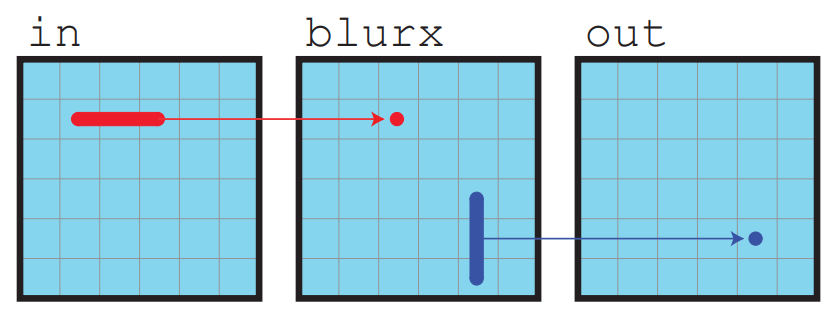
\includegraphics[width=3cm]{img/halide-breadth-first.png}
          \begin{itemize}
            \item[\xmark\xmark] Producer-consumer locality
            \item[\cmark\cmark] Parallelization
            \item[\cmark\cmark] Recomputation
          \end{itemize}
        \end{subfigure}
        \begin{subfigure}[H]{.31\textwidth}
          \centering
          Total fusion/inline strategy
          \inputminted[tabsize=2,frame=single,rulecolor=gray,fontsize=\fontsize{4.2}{3}]{cpp}{fig/blur_3x3_total_fusion.cpp}
          \vspace{0.3cm}
          \centering
          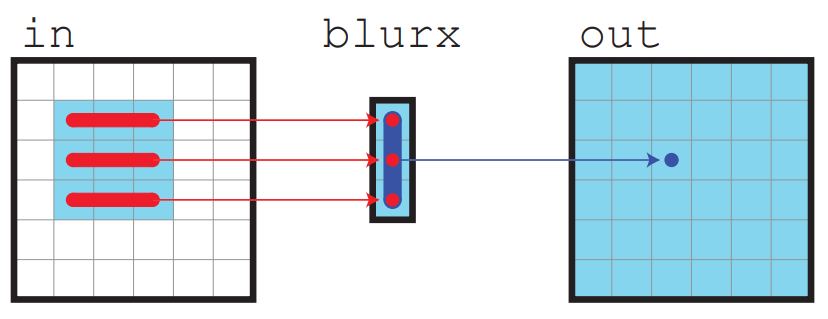
\includegraphics[width=3cm]{img/halide-total-fusion.png}
          \begin{itemize}
            \item[\cmark\cmark] Producer-consumer locality
            \item[\cmark\cmark] Parallelization
            \item[\xmark\xmark] Recomputation
          \end{itemize}
        \end{subfigure}
        \begin{subfigure}[H]{.3475\textwidth}
          \centering
          Sliding window strategy
          \inputminted[tabsize=2,frame=single,rulecolor=gray,fontsize=\fontsize{4.2}{3}]{cpp}{fig/blur_3x3_sliding_window.cpp}
          \centering
          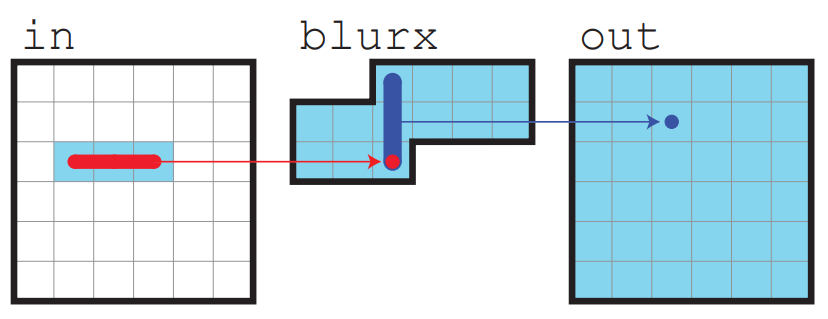
\includegraphics[width=3cm]{img/halide-sliding-window.png}
          \begin{itemize}
            \item[\cmark\cmark] Producer-consumer locality
            \item[\xmark\xmark] Parallelization
            \item[\cmark\cmark] Recomputation
          \end{itemize}
        \end{subfigure}
      \end{minipage}
    }
    \centering
    \unskip
    \vspace{0.3cm}
    \begin{tikzpicture}
      \coordinate (a) at (0cm,0cm);
      \coordinate (b) at (1.5cm,0);
      \coordinate (c) at (60:1.5cm);
      %
      \draw[color=black, fill=gray!40] (a) -- (b) -- (c) -- cycle;
      %
      \node[right = 0.1cm of b] {redundant work};
      \node[left = 0.1cm of a] {locality};
      \node[above = 0.1cm of c] {parallelism};
      \node[align=center] at (0.75cm, 0.4cm) {\tiny tradeoff\\\tiny space};
    \end{tikzpicture}
  \end{figure}
\end{frame}

\begin{frame}[fragile]{Scheduling trade-offs (2)}
  \fontsize{6pt}{7.2}\selectfont
  \vspace{0.25cm}
  \begin{figure}[H]
    \makebox[\linewidth]{
      \begin{minipage}{\textwidth}
        \centering
        \begin{subfigure}[H]{.45\textwidth}
          \centering
          Tiling strategy
          \inputminted[tabsize=2,frame=single,rulecolor=gray,fontsize=\fontsize{4.2}{3}]{cpp}{fig/blur_3x3_tiling.cpp}
          \centering
          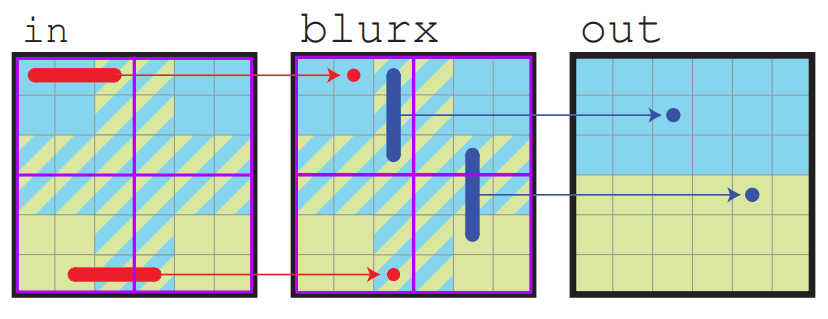
\includegraphics[width=3cm]{img/halide-tiling.png}
          \begin{itemize}
            \item[\cmark] Producer-consumer locality
            \item[\cmark\cmark] Parallelization
            \item[\xmark] Recomputation
          \end{itemize}
        \end{subfigure}
        \begin{subfigure}[H]{.45\textwidth}
          \centering
          Sliding window within tiling strategy
          \inputminted[tabsize=2,frame=single,rulecolor=gray,fontsize=\fontsize{4.2}{3}]{cpp}{fig/blur_3x3_sliding_window_tiling.cpp}
          \vspace{0.4cm}
          \centering
          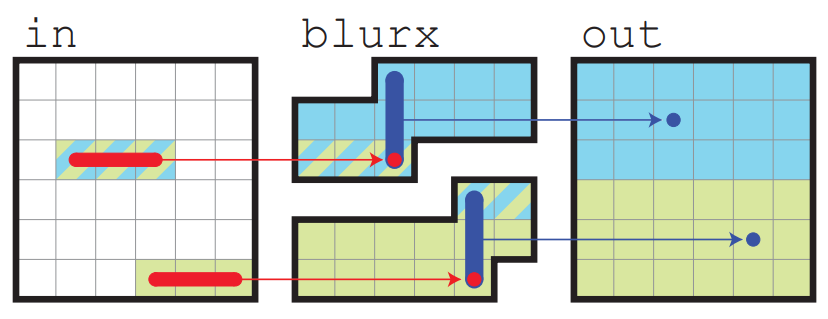
\includegraphics[width=3cm]{img/halide-sliding-window-tiling.png}
          \begin{itemize}
            \item[\cmark] Producer-consumer locality
            \item[\cmark] Parallelization
            \item[\cmark] Recomputation
          \end{itemize}
        \end{subfigure}
      \end{minipage}
    }
  \end{figure}
  \vspace{0.75cm}
  \metroset{block=fill}
  \begin{exampleblock}{Note}
    The best scheduling choice differs depending on each target architecture and the computational characteristics of the image pipeline stages.
  \end{exampleblock}
\end{frame}

\begin{frame}{Halide scheduling example}
  \fontsize{6pt}{7.2}\selectfont
  \begin{enumerate}
    \item Function's \textit{domain} is \textit{tiled} into $64\times64$-sized tiles
    \item Outer two loops of \textit{tiling} are \textit{fused} together into a single loop (\code{tile_index})
    \item \textit{Fused} loop is \textit{parallelized}
    \item Each \textit{tile} is \textit{tiled} again with $4\times2$-sized sub-tiles
    \item Sub-tile innermost $x$-loop (\code{x_vectors}) is \textit{vectorized} with the same factor as \code{x_vectors} ($4$): no iterations will be performed at this nesting level, the whole loop will be vectorized
    \item Sub-tile $y$-loop (\code{y_pairs}) is fully \textit{unrolled} with a factor matching the sub-tile vertical size ($2$), therefore eliminating the sub-tile inner loops in favor of \textit{unrolling} and \textit{vectorization}
  \end{enumerate}

  \begin{figure}[H]
    \begin{minipage}{0.6\textwidth}
      \centering
      \inputminted[tabsize=2,frame=single,rulecolor=gray,fontsize=\fontsize{5}{5}]{cpp}{fig/halide_scheduling_example.cpp}
    \end{minipage}
  \end{figure}
\end{frame}

\begin{frame}{Halide compilation flow}
  \fontsize{6pt}{7.2}\selectfont
  \begin{enumerate}
    \item \textbf{Lowering and loop synthesis}: given the \textit{schedule}, it generates the loop nests and allocations required to evaluate the pipeline, beginning from the output.
    \item \textbf{Bounds inference}: recursively back from the output and using interval analysis, for each function, it evaluates the bounds of the dimensions based on the bounds required by its caller and the indices it is called with.
    \item \textbf{Sliding window optimization and storage folding}: traverses the loop nests seeking opportunities for sliding window optimizations (when the results of a function are to be stored by a serial loop at a higher loop nesting level than its computation).
    \item \textbf{Flattening}: multi-dimensional loads, stores, and allocations are flattened into their linear single-dimensional equivalent.
    \item \textbf{Vectorization and unrolling}: converts loops that were scheduled as vectorized or unrolled into the corresponding loops. During vectorization, occurrences of a loop index are replaced with a special value $ramp(n)$ which represents the vector $[0, 1, \ldots, n-1]$.
    \item \textbf{Back-end code generation}: low-level optimizations are performed and machine code is emitted for the resulting pipeline. After running constant-folding and dead-code elimination passes, the Halide IR is ready to be lowered with a \code{CodeGen} backend. The primary backends use LLVM for code generation.
  \end{enumerate}

  \begin{figure}[H]
    \centering
    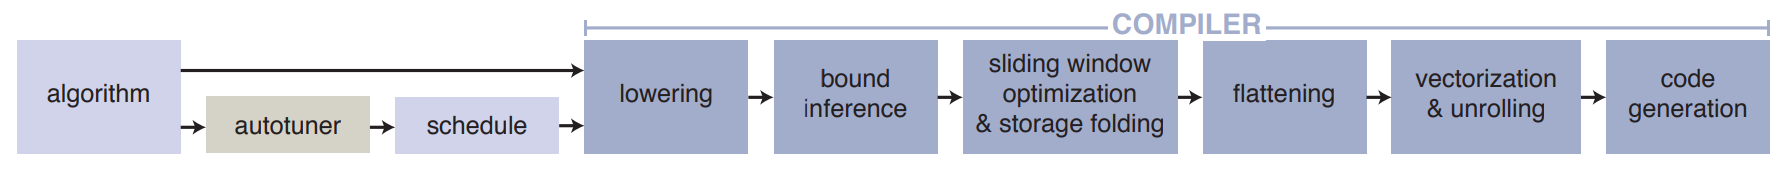
\includegraphics[width=\textwidth]{img/halide-compiler-flow.png}
  \end{figure}

\end{frame}

\begin{frame}{Halide IR}
  \begin{itemize}
    \item Halide IR nodes have an explicit type described by \codecpp{enum IRNodeType}. Examples:
          \begin{itemize}
            \item \codecpp{IntImm} to create integer immediates
            \item \code{Add} to represent additions
            \item \codecpp{Store} and \code{Load} to perform memory accesses
          \end{itemize}
    \item \codecpp{struct IRNode}: \codecpp{IRNodeType} + reference count. Virtual method \codecpp{accept} to implement the \textbf{visitor pattern}.
          \begin{itemize}
            \item \codecpp{IRVisitor}: traverse the IR nodes and perform some action on it (like generating code), but without modifying them.
            \item \codecpp{IRMutator}: traverse the IR nodes to modify them.
          \end{itemize}
    \item Two kinds of IR nodes, analogously to C:
          \begin{itemize}
            \item \textbf{Expressions} (\codecpp{ExprNode}): represent some value and have some type (e.g. \codecpp{x + 3})
            \item \textbf{Statements} (\codecpp{StmtNode}): side-effecting pieces of code that do not represent a value (e.g. \codecpp{assert(x > 3)}, \codecpp{store}).
          \end{itemize}
    \item Type system: signed and unsigned ints, IEEE fp numbers, opaque pointers (like \codecpp{void *}) and \code{bfloat}
  \end{itemize}
  \vspace*{0.1cm}
  \begin{figure}[H]
    \makebox[\linewidth]{
      \begin{minipage}[H]{\textwidth}
        \centering
        \begin{subfigure}[t]{.45\textwidth}
          \centering
          \codecpp{IntImm} node definition
          \inputminted[tabsize=2,frame=single,rulecolor=gray,fontsize=\fontsize{4.5}{4}]{cpp}{fig/halide_IntImm_node.cpp}
        \end{subfigure}
        \begin{subfigure}[t]{.475\textwidth}
          \centering
          \codecpp{IfThenElse} node definition
          \inputminted[tabsize=2,frame=single,rulecolor=gray,fontsize=\fontsize{4.5}{4}]{cpp}{fig/halide_IfThenElse_node.cpp}
          \vspace{0.4cm}
        \end{subfigure}
      \end{minipage}
    }
  \end{figure}
\end{frame}

\section{Multi-Level Intermediate Representation (MLIR)}

\begin{frame}{\raisebox{-0.25\height}{
\includegraphics[height=0.5cm]{img/mlir-identity-09.png}}}
  \begin{itemize}
    \item Multi-Level Intermediate Representation (MLIR): open-source compiler infrastructure project; provides common IR to represent \textbf{multiple levels of abstractions} maintaining a \textbf{unified interface}.
    \item Under LLVM's umbrella.
    \item Address challenges in building compilers and optimizing code generation for modern high-performance computing and machine-learning applications.
          \begin{itemize}
            \item Many compilation and system design problems are better modeled at a \textbf{higher-} or \textbf{lower-level abstraction}. Languages that use LLVM end up developing their IR to solve domain-specific problems. ML frameworks also use domain-specific abstractions (\textquote{ML graphs}).
            \item Makes it \textbf{easy} to define and \textbf{introduce new abstraction levels} and provides the infrastructure to use them to solve common compiler engineering problems.
          \end{itemize}
    \item MLIR infrastructure provides:
          \begin{enumerate}
            \item Standardized Static Single Assignment (\textbf{SSA})-based IR data structures.
            \item Declarative system for defining IR \textbf{dialects}.
            \item Wide range of common infrastructure: documentation, parsing and printing logic, multithreaded compilation support, \textbf{pass management}, etc.
          \end{enumerate}
  \end{itemize}
\end{frame}

\begin{frame}{\raisebox{-0.25\height}{
\includegraphics[height=0.5cm]{img/mlir-identity-09.png}} Dialects}
  \begin{itemize}
    \item \textbf{Dialect}: collection of related \textbf{operations}, \textbf{attributes} and \textbf{types} used to represent a particular domain.
          \begin{itemize}
            \item \textit{Attributes}: mechanism for specifying constant data on operations in places where a variable is never allowed (such as the comparison predicate of a \code{cmpi} operation).
          \end{itemize}
    \item MLIR allows for multiple dialects (even those outside of the main code tree) to \textbf{co-exist} together within one \textit{module}. Dialects are produced and consumed by certain \textbf{\textit{passes}}.
    \item Examples:
          \begin{itemize}
            \item \textbf{\textit{Arith}}: arithmetic dialect, holds basic integer and floating point mathematical operations which include: unary, binary, and ternary arithmetic ops, bitwise and shift ops, cast ops, and compare ops. Operations in this dialect also accept vectors and tensors of integers or floats.
            \item \textbf{\textit{Func}}: creation of high-level function abstractions and function calls.
            \item \textbf{\textit{Memref}}: memory reference, provides a collection of operations and types focused on representing and manipulating multi-dimensional arrays, or tensors, in memory.
            \item \textbf{\textit{SCF}}: structured control flow, which includes operations such as loops and conditionals.
            \item \textbf{\textit{Vector}}: supports multi-dimensional vector types and custom operations on them.
            \item \textbf{\textit{Affine}}: affine expressions and affine loops that allows polyhedral model compilation, analysis and optimizations.
          \end{itemize}
  \end{itemize}
\end{frame}

\begin{frame}{\raisebox{-0.25\height}{
\includegraphics[height=0.5cm]{img/mlir-identity-09.png}} IR}
  \begin{itemize}
    \item IR is \textbf{generic} enough to represent ASTs in a language frontend, generated instructions in a target-specific backend, HLS constructs, circuits (CIRCT), etc.
    \item IR is based on a graph-like data structure:
          \begin{itemize}
            \item Nodes: \textbf{\textit{Operations}}
            \item Edges: \textbf{\textit{Values}}
          \end{itemize}
          Each \textit{Value} is the result of exactly one \textit{Operation} or \textbf{\textit{Block Argument}} and has a \textbf{\textit{Value Type}} defined by the type system.
    \item Three forms: human-readable (\code{.mlir}), in-memory and serialized.
  \end{itemize}
  \begin{figure}[H]
    \centering
    \begin{minipage}{0.475\textwidth}
      \inputminted[tabsize=2,frame=single,rulecolor=gray,fontsize=\fontsize{6}{6}]{text}{fig/mlir_ir_example.mlir}
    \end{minipage}
  \end{figure}
\end{frame}

\section{Circuit IR Compilers and Tools (CIRCT)}

\begin{frame}{\raisebox{-0.25\height}{
\includegraphics[height=0.5cm]{img/circt-logo.png}} CIRCT}
  \begin{itemize}
    \item \textbf{C}ircuit \textbf{IR} \textbf{C}ompilers and \textbf{T}ools (CIRCT): project built \textbf{on top of MLIR}. Provides a set of tools and libraries to help with the \textbf{design} and verification of \textbf{digital circuits}.
    \item Adds new \textbf{hardware-oriented dialects} such as:
          \begin{itemize}
            \item \textit{\textbf{\code{hw}}}: generic HW dialect where other dialect operations are instantiated.
            \item \textit{\textbf{\code{comb}}}: models digital combinational logic.
            \item \textit{\textbf{\code{seq}}}: models digital sequential logic.
            \item \textit{\textbf{\code{fsm}}}: models finite-state machines.
            \item \textit{\textbf{\code{sv}}}: represents various SystemVerilog-specific constructs.
            \item \textit{\textbf{\code{calyx}}}: represents Calyx IR types and operations.
          \end{itemize}
    \item Provides a static scheduling infrastructure:
          \begin{itemize}
            \item A \textit{problem} is created from the IR (such as \textit{ModuloProblem}).
            \item A \textit{scheduler} solves the problem (list scheduler, LP-based schedulers, etc).
            \item \code{AffineToLoopSchedule} pass uses Calyx operator library for operation latencies and lowers to \code{LoopSchedule} dialect.
          \end{itemize}
    \item \codecpp{circt::createExportVerilogPass()} takes IR and emits SystemVerilog code.
          \begin{itemize}
            \item Style and options controlled by \codecpp{struct circt::LoweringOptions}.
          \end{itemize}
    \item Under LLVM's umbrella.
    \item SiFive contributing to CIRCT (order of magnitude faster than the current Chisel compiler).
  \end{itemize}
\end{frame}

\begin{frame}{\raisebox{-0.25\height}{
\includegraphics[height=0.5cm]{img/circt-logo.png}} CIRCT Dialects and conversion passes}
  \begin{figure}[H]
    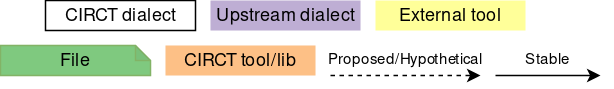
\includegraphics[width=4.1cm,left]{img/circt-dialectlegend.png}
  \end{figure}
  \begin{figure}[H]
    \centering
    \vspace*{-1.1cm}
    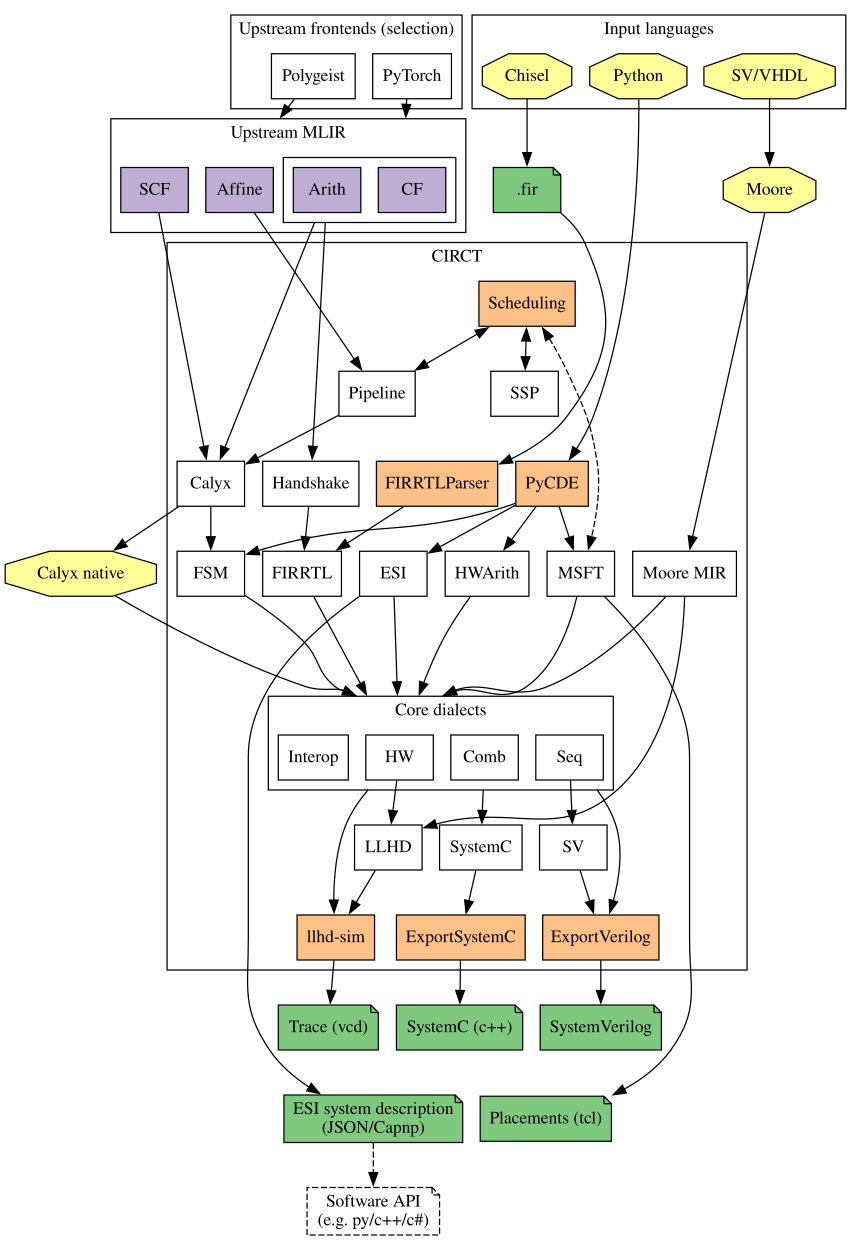
\includegraphics[height=8.1cm]{img/circt-dialects.png}
  \end{figure}
\end{frame}

\section{Calyx}

\begin{frame}[fragile]{\raisebox{-0.25\height}{
\includegraphics[height=0.5cm]{img/calyx-logo-text.png}}}
  \begin{itemize}
    \item Many hardware DSLs \textbf{re-engineer} a new \textbf{intermediate language} (IL) and compiler to generate the HW.
    \item \textbf{\textit{Calyx}} is a \textbf{shared IL} along a compiler infrastructure that implements useful optimizations and analyses, so that new hardware DSLs can use it as an \textbf{intermediate step} to quickly generate hardware designs.
    \item In Calyx, \textbf{\textit{components}} correspond to hardware modules (with input and output ports). Each \textit{component} has three distinct sections:
          \begin{itemize}
            \item \textbf{\code{cells}}: the instantion of hardware sub-components that form the \textit{component} being defined.
            \item \textbf{\code{wires}}: set of connection between the sub-components. They can be organized into \textbf{\code{groups}}.
            \item \textbf{\code{control}}: imperative control flow that defines the \textit{component}'s execution schedule (when each \code{group} executes).
          \end{itemize}
          \begin{figure}[H]
            \centering
            \begin{minipage}{0.32\textwidth}
              \inputminted[tabsize=2,frame=single,rulecolor=gray,fontsize=\fontsize{5}{5}]{text}{fig/calyx_component.calyx}
            \end{minipage}
          \end{figure}
    \item Each \code{group} has \textbf{\code{go}} and \textbf{\code{done}} ports. \code{go} triggers execution of the group, \code{done} finishes it. The \code{control} section uses those signals to orchestrate \code{group} execution.
    \item \code{Control} statements: \code{seq}, \code{par}, \code{if} and \code{while}.
    \item An \textit{assignment} can optionally have a \code{guard} expression:
          \begin{figure}[H]
            \centering
            \begin{minipage}{0.275\textwidth}
              \inputminted[tabsize=2,frame=single,rulecolor=gray,fontsize=\fontsize{5}{5}]{text}{fig/guarded_example.calyx}
            \end{minipage}
          \end{figure}
  \end{itemize}
\end{frame}

\section{Methodology}

\begin{frame}{Methodology}
  \begin{itemize}
    \item Converting Halide down to RTL (Xilinx FPGAs bitstream + XRT) is complex and involves \textbf{many steps}.
    \item \textbf{Top-down} and \textbf{incremental and iterative} design methodology. Start from simple Halide pipeline and keep adding complexity (new Halide IR nodes), then add MLIR conversion for them.
          \begin{itemize}
            \item Start with \codecpp{output(x) = x + 42;}, Halide IR nodes: \codecpp{Add}, \codecpp{IntImm}, \codecpp{For} and \codecpp{Store}.
          \end{itemize}
  \end{itemize}
  \begin{figure}
    \centering
    \scalebox{.36}{\begin{tikzpicture}[outerstyle/.style = {rectangle, draw, align=center}, innerstyle/.style = {rectangle, draw, align=center, fill=olive!30}, labelstyle/.style={draw=none, below right, inner sep=4pt}]
  \tikzstyle{every node}=[font=\large]
  % Halide
  \node[innerstyle, minimum width=4cm, style={fill=cyan!30}] (halide) {Halide IR};

  % CodeGen_MLIR
  \node[below=of halide] (empty0) {};
  \node[innerstyle, below=4mm of empty0] (mlir) {MLIR};
  \node[outerstyle, fit={(empty0) (mlir)}, below=of halide, minimum width=115mm] (CodeGen_MLIR) {};
  \node[labelstyle] at (CodeGen_MLIR.north west) {\code{CodeGen_MLIR}};

  % CodeGen_CIRCT
  \node[below=of mlir] (empty1) {};
  \node[innerstyle, below=4mm of empty1] (circt_calyx) {CIRCT (Calyx dialect)};
  \node[innerstyle, below=4mm of circt_calyx] (circt_hw) {CIRCT (HW dialects)};
  \node[outerstyle, fit={(empty1) (circt_calyx) (circt_hw)}, below=of mlir, minimum width=115mm] (CodeGen_CIRCT) {};
  \node[labelstyle] at (CodeGen_CIRCT.north west) {\code{CodeGen_CIRCT}};

  % CodeGen_CIRCT_Xilinx_Dev
  \node[below=of circt_hw] (empty2) {};
  \node[innerstyle, below=4mm of empty2] (circt_xilinx) {CIRCT (HW dialects)\\+\\Xilinx-specific RTL kernel wrappers};
  \node[outerstyle, fit={(empty2) (circt_xilinx)}, below=of circt_hw, minimum width=115mm] (CodeGen_CIRCT_Xilinx_Dev) {};
  \node[labelstyle] at (CodeGen_CIRCT_Xilinx_Dev.north west) {\code{CodeGen_CIRCT_Xilinx_Dev}};

  % ExportVerilog
  \node[below=of circt_xilinx] (empty3) {};
  \node[innerstyle, below=4mm of empty3] (sv_files) {SystemVerilog files};
  \node[outerstyle, fit={(empty3) (sv_files)}, below=of circt_xilinx, minimum width=115mm] (ExportVerilog) {};
  \node[labelstyle] at (ExportVerilog.north west) {\code{ExportVerilog}};

  % package_xo
  \node[below=of sv_files] (empty4) {};
  \node[innerstyle, below=4mm of empty4] (xo) {Xilinx object file (\code{.xo})};
  \node[outerstyle, fit={(empty4) (xo)}, below=of sv_files, minimum width=115mm] (package_xo) {};
  \node[labelstyle] at (package_xo.north west) {Xilinx Vivado \code{package_xo}};

  % v++
  \node[below=of xo] (empty5) {};
  \node[innerstyle, below=4mm of empty5] (xclbin) {Xilinx binary file (\code{.xclbin})};
  \node[outerstyle, fit={(empty5) (xclbin)}, below=of xo, minimum width=115mm] (v++) {};
  \node[labelstyle] at (v++.north west) {Xilinx Vitis \code{v++}};

  % XRT
  \node[below=of xclbin] (empty6) {};
  \node[innerstyle, below=4mm of empty6] (run) {Execute on the FPGA};
  \node[outerstyle, fit={(empty6) (run)}, below=of xclbin, minimum width=115mm] (XRT) {};
  \node[labelstyle] at (XRT.north west) {Halide XRT runtime (\code{xrt.cpp})};

  % arrows
  \draw [->] (halide.south) to (mlir);
  \draw [->] (mlir.south) to (circt_calyx);
  \draw [->] (circt_calyx.south) to (circt_hw);
  \draw [->] (circt_hw.south) to (circt_xilinx);
  \draw [->] (circt_xilinx.south) to (sv_files);
  \draw [->] (sv_files.south) to (xo);
  \draw [->] (xo.south) to (xclbin);
  \draw [->] (xclbin.south) to (run);

\end{tikzpicture}
}
  \end{figure}
\end{frame}

\section{Halide MLIR \textit{CodeGen}}

\begin{frame}{Marking loops to be offloaded to an accelerator}
  \begin{enumerate}
    \item \codecpp{InjectAcceleratorOffload} \codecpp{IRMutator} traverses IR and marks \code{For} IR nodes with new \codecpp{enum DeviceAPI::XRT}.
    \item For each marked \code{For} loop:
          \begin{enumerate}
            \item Pass the loop \codecpp{Stmt} and kernel name to virtual class called \codecpp{CodeGen_Accelerator_Dev}
                  \begin{itemize}
                    \item \codecpp{CodeGen_Xilinx_Dev} for \codecpp{enum DeviceAPI::XRT}
                  \end{itemize}
            \item Replace the loop with a call to the Halide runtime that has been implemented for XRT (\code{xrt.cpp}):
                  \begin{itemize}
                    \item \codecpp{halide_xrt_run} to start kernel execution
                    \item But also \codecpp{halide_xrt_initialize_kernels} and \codecpp{halide_xrt_finalize_kernels} before/after the kernel execution to load/unload the kernel (FPGA bitstream).
                  \end{itemize}
          \end{enumerate}
    \item \codecpp{CodeGen_Xilinx_Dev} uses \codecpp{CodeGen_MLIR} internally to generate the high-level MLIR code to be transformed into RTL.
  \end{enumerate}
\end{frame}

\begin{frame}{\code{CodeGen_MLIR}: Halide IR to MLIR conversion: Basics}
  \begin{itemize}
    \item Kernel arguments converted into \code{func}'s \codecpp{FuncOp}:
          \begin{itemize}
            \item Non-buffer arguments: \codecpp{mlir_type_of} converts Halide type to MLIR type.
            \item Buffer arguments: two MLIR arguments are generated:
                  \begin{enumerate}
                    \item 64-bit integer: base offset of the buffer within the assigned AXI interface. Written by the host code prior to kernel execution.
                    \item \codecpp{MemRefType} (\code{Memref} dialect): needed by MLIR to perform load/store accesses. Gets converted into a \textit{Calyx external memory interface} later on. Before accessing the base offset is added. Symbol name has \codecpp{".buffer"} suffix.
                  \end{enumerate}
          \end{itemize}
    \item Subclass of \codecpp{IRVisitor}, \codecpp{CodeGen_MLIR::Visitor}, walks IR tree and emits MLIR.
          \begin{itemize}
            \item Has a \codecpp{void visit(const <NodeType> *)} method for each Halide IR node type
          \end{itemize}
    \item \textquote{Scoped} symbol table maps string $\rightarrow$ \codecpp{mlir::Value}.
          \begin{itemize}
            \item \codecpp{sym_push}, \codecpp{sym_pop}, \codecpp{sym_get}
          \end{itemize}
    \item Helper methods \codecpp{codegen} for \codecpp{Expr} and \codecpp{Stmt}:
          \begin{figure}[H]
            \centering
            \begin{minipage}{0.3\textwidth}
              \inputminted[tabsize=2,frame=single,rulecolor=gray,fontsize=\fontsize{6}{6}]{cpp}{fig/codegen_methods.cpp}
            \end{minipage}
          \end{figure}
          They call \codecpp{accept} method of the \codecpp{Expr}/\codecpp{Stmt} passing \codecpp{this} as the \codecpp{IRVisitor*} argument, which calls the corresponding \codecpp{visit} method of the \codecpp{CodeGen_MLIR::Visitor} class for that \codecpp{Expr} or \codecpp{Stmt} node type.\\
          E.g. \codecpp{codegen(myIntImm)} calls \codecpp{IRVisitor::visit(const IntImm *)}.
  \end{itemize}
\end{frame}

\begin{frame}{\code{CodeGen_MLIR}: Halide IR to MLIR conversion: Basic nodes}
  \begin{itemize}
    \item \codecpp{Let}, \codecpp{LetStmt}: represent the \textquote{let} construct found in many functional programming languages.
          \begin{figure}[H]
            \centering
            \begin{minipage}{0.355\textwidth}
              \inputminted[tabsize=2,frame=single,rulecolor=gray,fontsize=\fontsize{5}{5}]{cpp}{fig/let_conversion.cpp}
            \end{minipage}
          \end{figure}
    \item \codecpp{IntImm}, \codecpp{UIntImm}, \codecpp{FloatImm}: numeric immediates. \codecpp{mlir_type_of} to convert it to the corresponding \codecpp{mlir::Type}.
          \begin{figure}[H]
            \centering
            \begin{minipage}{0.46\textwidth}
              \inputminted[tabsize=2,frame=single,rulecolor=gray,fontsize=\fontsize{5}{5}]{cpp}{fig/immediate_conversion.cpp}
            \end{minipage}
          \end{figure}
    \item \codecpp{Add}, \codecpp{Sub}: addition/subtraction of two \codecpp{Expr}.
          \begin{figure}[H]
            \centering
            \begin{minipage}{0.55\textwidth}
              \inputminted[tabsize=2,frame=single,rulecolor=gray,fontsize=\fontsize{5}{5}]{cpp}{fig/add_conversion.cpp}
            \end{minipage}
          \end{figure}
    \item \codecpp{EQ}, \codecpp{NE}: equality and inequality comparison operations.
          \begin{figure}[H]
            \centering
            \begin{minipage}{0.55\textwidth}
              \inputminted[tabsize=2,frame=single,rulecolor=gray,fontsize=\fontsize{5}{5}]{cpp}{fig/eq_conversion.cpp}
            \end{minipage}
          \end{figure}
  \end{itemize}
\end{frame}

\begin{frame}{\code{CodeGen_MLIR}: Halide IR to MLIR conversion: \code{For} loop}
  \begin{itemize}
    \item \codecpp{For}: the only loop construct that Halide IR has.
          \begin{figure}[H]
            \centering
            \begin{minipage}{0.65\textwidth}
              \inputminted[tabsize=2,frame=single,rulecolor=gray,fontsize=\fontsize{5}{5}]{cpp}{fig/for_conversion.cpp}
            \end{minipage}
          \end{figure}
  \end{itemize}
\end{frame}

\begin{frame}{\code{CodeGen_MLIR}: Halide IR to MLIR conversion: \code{Load}/\code{Store}}
  \begin{itemize}
    \item \codecpp{Load}, \codecpp{Store}: memory accesses.
          \begin{figure}[H]
            \centering
            \begin{minipage}{0.75\textwidth}
              \inputminted[tabsize=2,frame=single,rulecolor=gray,fontsize=\fontsize{5}{5}]{cpp}{fig/load_conversion.cpp}
            \end{minipage}
          \end{figure}
  \end{itemize}
\end{frame}

\section{Lowering MLIR to CIRCT}

\begin{frame}{\code{CodeGen_CIRCT}: Generates generic RTL kernel}
  \begin{itemize}
    \item \codecpp{MemRefType} arguments transformed into \textit{Calyx external memory interface}
    \item New features implemented:
          \begin{itemize}
            \item Passing custom argument names to Calyx
            \item Support for sequential-reads memories (\code{read_en}) and variable memory-access sizes (\code{access_size})
            \item Support more \code{arith} dialect operations such as \codecpp{MinSIOp}
            \item Adding initial vector support (\code{calyx::AssignOp} modified to assign flattened bits $\leftrightarrow$ vectors)
            \item Implement basic \code{vector} dialect operations (such as \codecpp{vector::SplatOp}, a scalar $\rightarrow$ vector broadcast)
          \end{itemize}
  \end{itemize}
  \begin{figure}
    \centering
    \scalebox{.4}{\begin{tikzpicture}[outerstyle/.style = {rectangle, draw, align=center}, innerstyle/.style = {rectangle, draw, align=center, fill=olive!30}, labelstyle/.style={draw=none, below right, inner sep=4pt}]

% Generic MLIR
\node[innerstyle, minimum width=4cm, style={fill=cyan!30}] (MLIR) {Generic MLIR};

% CodeGen_CIRCT
\node[below=6mm of MLIR] (empty1) {};
\node[below=of empty1] (empty2) {};

\node[innerstyle, below=4mm of empty2] (for_to_while) {\codecpp{mlir::createForToWhileLoopPass()}};
\node[innerstyle, below=4mm of for_to_while] (scf_to_calyx) {\codecpp{circt::createSCFToCalyxPass()}};

\node[below=of scf_to_calyx] (empty3) {};

\node[innerstyle, below=4mm of empty3] (remove_comb_groups) {\codecpp{circt::calyx::createRemoveCombGroupsPass()}};
\node[innerstyle, below=4mm of remove_comb_groups] (calyx_to_fsm) {\codecpp{circt::createCalyxToFSMPass()}};
\node[innerstyle, below=4mm of calyx_to_fsm] (materialize_calyx_fsm) {\codecpp{circt::createMaterializeCalyxToFSMPass()}};
\node[innerstyle, below=4mm of materialize_calyx_fsm] (remove_groups_from_fsm) {\codecpp{circt::createRemoveGroupsFromFSMPass()}};
\node[innerstyle, below=4mm of remove_groups_from_fsm] (clk_ins) {\codecpp{circt::calyx::createClkInsertionPass()}};
\node[innerstyle, below=4mm of clk_ins] (reset_ins) {\codecpp{circt::calyx::createResetInsertionPass()}};
\node[innerstyle, below=4mm of reset_ins] (calyx_to_hw) {\codecpp{circt::createCalyxToHWPass()}};

\node[below=4mm of calyx_to_hw] (empty4) {};
\node[below=4mm of empty4] (empty5) {};

\node[outerstyle, fit={(empty2) (for_to_while) (scf_to_calyx)}, below=of empty1, minimum width=105mm] (MLIR_to_Calyx) {};

\node[outerstyle, fit={(empty3) (remove_comb_groups) (calyx_to_fsm) (materialize_calyx_fsm) (remove_groups_from_fsm) (clk_ins) (reset_ins) (calyx_to_hw)}, below=of scf_to_calyx, minimum width=105mm] (Calyx_to_HW) {};

\node[outerstyle, fit={(MLIR_to_Calyx) (Calyx_to_HW) (empty5)}, below=of MLIR, minimum width=115mm] (CodeGen_CIRCT) {};

\node[labelstyle] at (MLIR_to_Calyx.north west) {MLIR to Calyx};
\node[labelstyle] at (Calyx_to_HW.north west) {Calyx to hardware};
\node[labelstyle] at (CodeGen_CIRCT.north west) {\code{CodeGen_CIRCT}};

% XRT
\node[innerstyle, below=10mm of empty4, style={fill=cyan!30}] (circt_hw_dialects) {CIRCT with hardware dialects};

% arrows
\draw [->] (MLIR.south) to (for_to_while);
\draw [->] (for_to_while.south) to (scf_to_calyx);
\draw [->] (scf_to_calyx.south) to (remove_comb_groups);
\draw [->] (remove_comb_groups.south) to (calyx_to_fsm);
\draw [->] (calyx_to_fsm.south) to (materialize_calyx_fsm);
\draw [->] (materialize_calyx_fsm.south) to (remove_groups_from_fsm);
\draw [->] (remove_groups_from_fsm.south) to (clk_ins);
\draw [->] (clk_ins.south) to (reset_ins);
\draw [->] (reset_ins.south) to (calyx_to_hw);
\draw [->] (calyx_to_hw.south) to (circt_hw_dialects);

\end{tikzpicture}
}
  \end{figure}
\end{frame}

\section{Wrapping the generic RTL kernel for Xilinx FPGAs}

\begin{frame}{CIRCT to Xilinx RTL}
  \begin{itemize}
    \item Wraps generic RTL kernel with necessary Xilinx-specific logic: \textit{Calyx external memory} to AXI converters and AXI4-Lite subordinate \textbf{control logic} specified by XRT.
    \item Generates SystemVerilog code and \code{kernel.xml} file needed by Vitis \code{v++}.
  \end{itemize}
  \begin{figure}
    \centering
    \scalebox{.4}{\begin{tikzpicture}[outerstyle/.style = {rectangle, draw, align=center}, innerstyle/.style = {rectangle, draw, align=center, minimum height=6mm,  fill=olive!30}, labelstyle/.style={draw=none, below right, inner sep=4pt}]

% Generic MLIR
\node[innerstyle, minimum width=4cm, style={fill=cyan!30}] (MLIR) {CIRCT with hardware dialects};

% CodeGen_CIRCT_Xilinx_Dev
\node[below=6mm of MLIR] (empty1) {};
\node[below=of empty1] (empty2) {};

\node[innerstyle, below=4mm of empty2] (add_calyx_ext_mem_to_axi) {Add Calyx external memory to AXI converters};
\node[innerstyle, below=4mm of add_calyx_ext_mem_to_axi] (add_control) {Add AXI4-Lite kernel control interface};
\node[innerstyle, below=4mm of add_control] (add_toplevel) {Add top-level};

\node[below=of add_toplevel] (empty3) {};

\node[innerstyle, below=4mm of empty3] (seq_to_hlmem) {\codecpp{circt::seq::createLowerSeqHLMemPass()}};
\node[innerstyle, below=4mm of seq_to_hlmem] (fsm_to_sv) {\codecpp{circt::createConvertFSMToSVPass()}};
\node[innerstyle, below=4mm of fsm_to_sv] (seq_to_sv) {\codecpp{circt::seq::createSeqLowerToSVPass()}};
\node[innerstyle, below=4mm of seq_to_sv] (export_sv) {\codecpp{circt::exportSplitVerilog(directory)}};

\coordinate (export_sv_midsw) at ($(export_sv.south west)!.5!(export_sv.south)$);

\node[below=4mm of export_sv_midsw] (empty4) {};
\node[innerstyle, below=9mm of export_sv, anchor=west] (gen_kernelxml) {Generate \code{kernel.xml}};
\node[below=7mm of gen_kernelxml] (empty5) {};
\node[below=4mm of empty5] (empty6) {};

\node[outerstyle, fit={(empty2) (add_calyx_ext_mem_to_axi) (add_control) (add_toplevel)}, below=of empty1, minimum width=105mm] (add_xilinx_wrappers) {};

\node[outerstyle, fit={(empty3) (seq_to_hlmem) (fsm_to_sv) (seq_to_sv) (export_sv)}, below=of add_toplevel, minimum width=105mm] (Generate_SV) {};

\node[outerstyle, fit={(add_xilinx_wrappers) (Generate_SV) (gen_kernelxml) (empty5)}, below=of MLIR, minimum width=115mm] (CodeGen_CIRCT_Xilinx_Dev) {};

\node[labelstyle] at (add_xilinx_wrappers.north west) {Add Xilinx wrappers};
\node[labelstyle] at (Generate_SV.north west) {Generate SystemVerilog};
\node[labelstyle] at (CodeGen_CIRCT_Xilinx_Dev.north west) {\code{CodeGen_CIRCT_Xilinx_Dev}};

% SV
\node[innerstyle, below=18mm of empty4, style={fill=cyan!30}] (sv_code) {SystemVerilog code};

% kernel.xml
\node[innerstyle, below=12.6mm of gen_kernelxml, style={fill=cyan!30}] (kernel_xml) {\code{kernel.xml}};

% arrows
\draw [->] (MLIR.south) to (add_calyx_ext_mem_to_axi);
\draw [->] (add_calyx_ext_mem_to_axi.south) to (add_control);
\draw [->] (add_control.south) to (add_toplevel);
\draw [->] (add_toplevel.south) to (seq_to_hlmem);
\draw [->] (seq_to_hlmem.south) to (fsm_to_sv);
\draw [->] (fsm_to_sv.south) to (seq_to_sv);
\draw [->] (seq_to_sv.south) to (export_sv);
\draw [->] (export_sv_midsw) to (sv_code);
\draw [->] (gen_kernelxml.south) to (kernel_xml);

\end{tikzpicture}
}
  \end{figure}
\end{frame}

\begin{frame}{\textit{Calyx external memory} to AXI converter}
  \begin{itemize}
    \item Buffer kernel arguments are accessed through \textit{Calyx external memory interface}.
          \begin{itemize}
            \item Each buffer is mapped into a different interface. This module converts it to AXI.
          \end{itemize}
    \item FSM handles two-way handshake of AXI transfers.
  \end{itemize}
  \begin{figure}[H]
    \begin{minipage}[H]{\textwidth}
      \centering
      \begin{subfigure}[t]{.45\textwidth}
        \centering
        \scalebox{.6}{\begin{tikzpicture}[node distance = 4mm and 4mm, every node/.style={scale=0.75}]
\node (mod) [draw, minimum width=48mm, minimum height=70mm, align=center] at (0,0) {Calyx external memory\\to AXI converter};
%
\coordinate[above left = 22mm and 14mm of mod.west]   (a1);
\foreach \i [count=\xi from 1] in {2,...,13}
  \coordinate[below=of a\xi]  (a\i);
%
\coordinate[above right = 24mm and 14mm of mod.east]  (b1);
\foreach \i [count=\xi from 1] in {2,...,13}
  \coordinate[below=of b\xi]  (b\i);
%
\foreach \i [count=\xi from 1] in {
  \code{m_axi_arready},
  \code{m_axi_rdata},
  \code{m_axi_rvalid},
  \code{m_axi_rlast},
  \code{m_axi_awready},
  \code{m_axi_wready},
  \code{m_axi_bvalid}
}
  \draw[->]  (a\xi) node[left, text=blue] {\i} -- (a\xi-| mod.west);

\foreach \i [count=\xi from 8] in {
  \code{calyx_write_data},
  \code{calyx_addr0},
  \code{calyx_write_en},
  \code{calyx_read_en},
  \code{calyx_access_size}
}
  \draw[->]  (a\xi) node[left, text=red] {\i} -- (a\xi-| mod.west);

\foreach \i [count=\xi from 1] in {
  \code{m_axi_arvalid},
  \code{m_axi_arlen},
  \code{m_axi_rready},
  \code{m_axi_awaddr},
  \code{m_axi_awvalid},
  \code{m_axi_awlen},
  \code{m_axi_wdata},
  \code{m_axi_wvalid},
  \code{m_axi_wstrb},
  \code{m_axi_wlast},
  \code{m_axi_bready}
}
  \draw[->] (mod.east |- b\xi) -- (b\xi) node[right, text=blue] {\i};

\foreach \i [count=\xi from 12] in {
  \code{calyx_read_data},
  \code{calyx_done}
}
  \draw[->] (mod.east |- b\xi) -- (b\xi) node[right, text=red] {\i};

\end{tikzpicture}
}
        \caption{\textit{Calyx external memory} to AXI converter}
      \end{subfigure}
      \begin{subfigure}[t]{.45\textwidth}
        \centering
        \scalebox{.5}{\begin{tikzpicture}[shorten >=1pt, auto, node distance=4.2cm, scale=0.75, transform shape, state/.style={circle split, draw, minimum size=2.3cm}]
\node[state, initial, style={circle}] (IDLE) {IDLE};
\node[state] (AW)     [right of=IDLE] {AW      \nodepart{lower} \code{awvalid=1}};
\node[state] (W)      [right of=AW]   {W       \nodepart{lower} \code{wvalid=1}};
\node[state] (B_WAIT) [right of=W]    {B\_WAIT \nodepart{lower} \code{bready=1}};
\node[state] (AR)     [below of=IDLE, node distance=5cm] {AR      \nodepart{lower} \code{arvalid=1}};
\node[state] (R)      [below of=W]    {R       \nodepart{lower} \code{rready=1}};
\path[-{Stealth[black]}]
(IDLE) edge [text=red, bend left]        node {\code{calyx_write_en}} (AW)
(IDLE) edge [text=red, bend right, left] node {\code{calyx_read_en}} (AR)
(AW) edge [text=blue, bend left]         node {\code{m_axi_awready}} (W)
(W) edge [text=blue, bend left]          node {\code{m_axi_wready}} (B_WAIT)
(B_WAIT) edge [bend left]     node {\textcolor{blue}{\code{m_axi_bvalid}} / \textcolor{red}{\code{calyx_done}}} (IDLE)
(AR) edge [text=blue, bend right, below] node {\code{m_axi_arready}} (R)
(R) edge [bend right=-18]     node {\makecell[c]{\textcolor{blue}{\code{m_axi_rvalid}} \\ / \\ \textcolor{red}{\code{calyx_done}}}} (IDLE);
\end{tikzpicture}
}
        \caption{\textit{Calyx external memory} to AXI converter FSM}
      \end{subfigure}
    \end{minipage}
  \end{figure}
\end{frame}

\begin{frame}{Kernel control logic}
  \begin{itemize}
    \item Support seamless integration with Xilinx runtime libraries: XRT-managed kernel control requirements.
    \item Kernel acts as an AXI4-Lite subordinate and exposes a set of registers that are used by the host to control the kernel execution and set up the kernel.
          \begin{itemize}
            \item Control register with \code{start} and \code{done} bits.
            \item Interrupt registers to enable/mask interrupts.
            \item At offset \codecpp{+0x10} kernel arguments.
          \end{itemize}
    \item Interrupt line signals events kernel $\rightarrow$ host to avoid continuous polling.
  \end{itemize}
  \begin{figure}[H]
    \begin{minipage}[H]{\textwidth}
      \centering
      \begin{subfigure}[t]{.45\textwidth}
        \centering
        \scalebox{.5}{\begin{tikzpicture}[shorten >=1pt, auto, node distance=5cm, scale=0.75, transform shape, state/.style={circle split, draw, minimum size=2.3cm}]
\node[state, initial] (IDLE)                 {IDLE \nodepart{lower} \code{arready=1}};
\node[state]          (DATA) [right of=IDLE] {DATA \nodepart{lower} \code{rvalid=1}};
\path[-{Stealth[black]}]
(IDLE) edge [bend left] node {\code{s_axi_control_arvalid}} (DATA)
(DATA) edge [bend left] node {\code{s_axi_control_rready}}  (IDLE);
\end{tikzpicture}
}
        \caption{Control interface read handler FSM.}
      \end{subfigure}
      \begin{subfigure}[t]{.45\textwidth}
        \centering
        \scalebox{.5}{\begin{tikzpicture}[shorten >=1pt, auto, node distance=5cm, scale=0.75, transform shape, state/.style={circle split, draw, minimum size=2.3cm}]
\node[state, initial] (IDLE)                 {IDLE \nodepart{lower} \code{awready=1}};
\node[state]          (DATA) [right of=IDLE] {DATA \nodepart{lower} \code{wready=1}};
\node[state]          (RESP) [right of=DATA] {RESP \nodepart{lower} \code{bvalid=1}};
\path[-{Stealth[black]}]
(IDLE) edge [bend left] node {\code{s_axi_control_awvalid}} (DATA)
(DATA) edge [bend left] node {\code{s_axi_control_wvalid}}  (RESP)
(RESP) edge [bend left] node {\code{s_axi_control_bready}}  (IDLE);
\end{tikzpicture}
}
        \caption{Control interface write handler FSM.}
      \end{subfigure}
    \end{minipage}
  \end{figure}
\end{frame}

\section{Halide runtime XRT backend}

\begin{frame}{Halide runtime XRT backend (\code{xrt.cpp})}
  \begin{itemize}
    \item Implements \codecpp{struct halide_device_interface_impl_t} interface:
          \begin{itemize}
            \item \codecpp{halide_xrt_device_malloc}: allocate buffers that the device can access.
            \item \codecpp{halide_xrt_device_free}: deallocate them.
            \item \codecpp{halide_xrt_copy_to_device}: copy a buffer to device/flush CPU cache so that all changes are visible to the device.
            \item \code{halide_xrt_copy_to_host}: copy buffer to host/flush all the relevant device buffers and invalidate CPU cache so that all changes are visible to the host.
          \end{itemize}
    \item Also implements functions called directly when \code{For} loop is offloaded to the accelerator:
          \begin{itemize}
            \item \codecpp{halide_xrt_initialize_kernels}: loads a kernel into the device.
            \item \codecpp{halide_xrt_finalize_kernels}: unload the kernel.
            \item \codecpp{halide_xrt_run}: starts kernel execution with the specified arguments.
          \end{itemize}
    \item Allocating buffers depends on loading kernel first, so they are \textbf{lazily allocated}: just prior to kernel execution.
    \item Uses XRT's C API. Seamless integration with Halide.
  \end{itemize}
\end{frame}

\section{Bugs and issues}

\begin{frame}[fragile]{Bugs and issues}
  \begin{itemize}
    \item MLIR and CIRCT are still experimental projects.
    \item MLIR SCF $\rightarrow$ Calyx pass and Calyx $\rightarrow$ HW dialects had \textbf{never been tested on real hardware} (or even cycle-accurate simulator)
    \item Numerous bugs were found. Waveform debugging was essential.
    \item Bugs were fixed, submitted to upstream, and already merged:
          \begin{itemize}
            \item Add support for multiple \codecpp{calyx::AssignOp} with guards to the same destination
                  \begin{figure}
                    \scalebox{.5}{\begin{tikzpicture}[node distance=0.5cm and 0.5cm]
\tikzset{mux 2by1/.style={muxdemux,muxdemux def={Lh=2, NL=2, Rh=1,NB=0,NT=1, w=1}}}
  \node [font=\small] (G0) at (0,0) {$guard_0$};
  \node [font=\small] (G1) at (2,0) {$guard_1$};
  \node [font=\small] (GN) at (4,0) {$guard_N$};

  \node [mux 2by1] (M0) [below of=G0, anchor=tpin 1] {};
  \node [mux 2by1] (M1) [below of=G1, anchor=tpin 1] at (2,-0.5) {};
  \node [mux 2by1] (MN) [below of=GN, anchor=tpin 1] at (4,-1.0) {};

  \foreach \i in {0,1,N} {
    \foreach \x [count=\c] in {0,...,1} {
      \node [right, font=\tiny] at ($(M\i.lpin \c)+(0.2,0)$) {\x};
    }
    \draw (M\i.tpin 1) |- (G\i.south);
    \node [left, font=\small] at (M\i.lpin 2) {$in_\i$};
  }
  \draw (M0.rpin 1) |- (M1.lpin 1);
  \draw[thick, dotted] (M1.rpin 1) |- (MN.lpin 1);

  \node [left, font=\small] at (M0.lpin 1) {$0$};
  \node [right, font=\small] at (MN.rpin 1) {$out$};
\end{tikzpicture}
}
                  \end{figure}
            \item Clock-enable with the \code{done} signal when writing to Calyx registers
                  \begin{figure}[H]
                    \centering
                    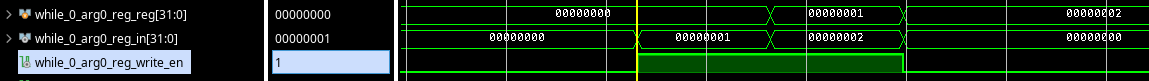
\includegraphics[width=8cm,valign=b]{img/bug_write_en_done.png}
                    $\implies$
                    \adjustbox{valign=c}{\scalebox{.5}{\begin{tikztimingtable}[timing/inline node/.style={coordinate,shift={(0.05, 0.5)}}]
  clock                                   & 10{2C}G          \\
  \code{write_en}\textsubscript{\code{B}} & 6C8C6C           \\
  \code{done_reg}\textsubscript{\code{B}} & 10C N(A) 10C           \\
  \code{clock_en}\textsubscript{\code{B}} & 6C4C10C          \\
  FSM state                               & 6D{[teal,font=\bfseries]A}8D{[blue,font=\bfseries]B} N(B) 6D{[red,font=\bfseries]C}  \\
  \extracode
    \vertlines[help lines,opacity=0.4]{2,6,10,14,18}
    \draw[orange, semithick]
      (A) ellipse (.4 and .8) +(0, -0.8) coordinate (Ax)
      (B) ellipse (.4 and .8) +(0, +0.8) coordinate (Bx);
    \draw [orange, semithick, ->]
      (Ax) parabola [bend pos=0.5] (Bx);
\end{tikztimingtable}
}}
                  \end{figure}
            \item \codecpp{calyx::NotLibOp} was lowered incorrectly (\textit{XOR} with 0s instead of 1s)
            \item Read/write-enable signals of external memories were left unconnected
          \end{itemize}
  \end{itemize}
\end{frame}

\section{Evaluation}

\begin{frame}{Evaluation}
  \begin{itemize}
    \item Avnet Ultra96-V2 Board with 2 GB LPDDR4:
          \begin{table}[H]
            \centering
            \scalebox{.5}{\begin{tabular}{|c|c|}
\hline
\textbf{Processor Core} & Quad-core Arm® Cortex®-A53 MPCore™ up to 1.5GHz \\
\hline
\textbf{Memory w/ECC} & L1 Cache 32KB I/D per core, L2 Cache 1MB, on-chip Memory 256KB \\
\hline
\textbf{Graphics Processing Unit} & Mali™-400 MP2 up to 667MHz \\
\hline
\textbf{Memory} & L2 Cache 64KB \\
\hline
\textbf{DRAM Interface} & x16: DDR4 w/o ECC; x32/x64: DDR4, LPDDR4, DDR3, DDR3L, LPDDR3 w/ ECC \\
\hline
\textbf{High-Speed Connectivity} & PCIe® Gen2 x4, 2x USB3.0, SATA 3.1, DisplayPort, 4x Tri-mode Gigabit Ethernet \\
\hline
\end{tabular}
}
            \scalebox{.5}{\begin{tabular}{|c|c|c|}
\hline
\multirow{3}{*}{Programmable Functionality} &
    \textbf{System Logic Cells (K)} & 154 \\
    \arrayrulecolor{gray!40}\cline{2-3}\arrayrulecolor{black} &
    \textbf{CLB Flip-Flops (K)}     & 141 \\
    \arrayrulecolor{gray!40}\cline{2-3}\arrayrulecolor{black} &
    \textbf{CLB LUTs (K)}                  & 71 \\
\hline
\multirow{3}{*}{Memory} &
    \textbf{Max. Distributed RAM (Mb)}     & 1.8 \\
    \arrayrulecolor{gray!40}\cline{2-3}\arrayrulecolor{black} &
    \textbf{Total Block RAM (Mb)}          & 7.6 \\
    \arrayrulecolor{gray!40}\cline{2-3}\arrayrulecolor{black} &
    \textbf{UltraRAM (Mb)}                 & - \\
\hline
\multirow{1}{*}{Clocking} &
    \textbf{Clock Management Tiles (CMTs)} & 3 \\
\hline
\multirow{1}{*}{Integrated IP} &
    \textbf{DSP Slices}                   & 360 \\
\hline
\end{tabular}
}
          \end{table}
    \item 3 Halide kernels used to evaluate the generated RTL code
    \item For each kernel, resource utilization and execution time analysis performed
    \item Each kernel has been run three times and the average time has been taken
    \item The result (output data) of RTL execution binary-compared with CPU execution (\textquote{golden model})
          \begin{itemize}
            \item Timing of CPU execution taken with vanilla kernel without Halide scheduling directives (defaults to \textit{inline}/\textit{total fusion})
          \end{itemize}
    \item For all the kernels, the ${\SI{150}{\mega\hertz}}$ target frequency was met.
          \begin{itemize}
            \item Note: ${\SI{150}{\mega\hertz}}$ on the FPGA, while the CPU runs at ${\SI{1.5}{\giga\hertz}}$, 10 times faster
          \end{itemize}
  \end{itemize}

\end{frame}

\begin{frame}{\textit{Test load} kernel}
  \begin{itemize}
    \item Tests the load and store from external memory functionality (32-bit ints):
          \begin{figure}[H]
            \centering
            \begin{minipage}{0.3\textwidth}
              \inputminted[tabsize=2,frame=single,rulecolor=gray,fontsize=\fontsize{5}{5}]{cpp}{fig/test_load_kernel.cpp}
            \end{minipage}
          \end{figure}
    \item Evaluation: vect. factors: powers of two from 1 to 32. AXI data bus widths: vector size and max (1024).
    \item Resource usage:
          \begin{table}[Ht]
            \makebox[\linewidth]{
              \scalebox{.333}{\begin{tabular}{|c|c|c|c|c|c|c|c|c|c|c|c|}
\cline{2-12}
\multicolumn{1}{c|}{} & \multicolumn{11}{c|}{\textbf{Vectorization factor}} \\
\cline{2-12}
\multicolumn{1}{c|}{} & \multicolumn{2}{c|}{\textbf{None (1)}} & \multicolumn{2}{c|}{\textbf{2}} & \multicolumn{2}{c|}{\textbf{4}} & \multicolumn{2}{c|}{\textbf{8}} & \multicolumn{2}{c|}{\textbf{16}} & \multicolumn{1}{c|}{\textbf{32}} \\
\hline
\multicolumn{1}{|c|}{\textbf{AXI data bus size (bits)}} & 32 & 1024 & 64 & 1024 & 128 & 1024 & 256 & 1024 & 512 & 1024 & 1024 \\
\hline
\multicolumn{1}{|l|}{CLB LUTs}                        & 39.29 & 50.55 & 39.61 & 50.75 & 39.09 & 51.65 & 42.65 & 53.50 & 47.58 & 55.52 & 58.21 \\
\grayline
\multicolumn{1}{|l|}{\hspace{25pt}LUT as Logic}       & 35.65 & 46.88 & 35.97 & 47.09 & 35.51 & 47.98 & 39.01 & 49.84 & 43.91 & 51.85 & 54.55 \\
\grayline
\multicolumn{1}{|l|}{\hspace{25pt}LUT as Memory}      &  8.92 &  8.98 &  8.92 &  8.98 &  8.76 &  8.98 &  8.93 &  8.98 &  8.98 &  8.98 &  8.98 \\
\hline
\multicolumn{1}{|l|}{CLB Registers}                   & 28.81 & 39.36 & 29.43 & 39.41 & 30.00 & 39.50 & 32.09 & 39.69 & 35.00 & 40.05 & 40.78 \\
\grayline
\multicolumn{1}{|l|}{\hspace{25pt}Register as FF}     & 28.79 & 39.34 & 29.41 & 39.39 & 29.98 & 39.47 & 32.07 & 39.66 & 34.97 & 40.02 & 40.75 \\
\grayline
\multicolumn{1}{|l|}{\hspace{25pt}Register as Latch}  &  0.02 &  0.02 &  0.02 &  0.03 &  0.02 &  0.03 &  0.03 &  0.03 &  0.03 & 0.03 &  0.03 \\
\hline
\end{tabular}
}
              \scalebox{.333}{\begin{tabular}{|c|c|c|c|c|c|c|c|c|c|c|c|}
\cline{2-12}
\multicolumn{1}{c|}{} & \multicolumn{11}{c|}{\textbf{Vectorization factor}} \\
\cline{2-12}
\multicolumn{1}{c|}{} & \multicolumn{2}{c|}{\textbf{None (1)}} & \multicolumn{2}{c|}{\textbf{2}} & \multicolumn{2}{c|}{\textbf{4}} & \multicolumn{2}{c|}{\textbf{8}} & \multicolumn{2}{c|}{\textbf{16}} & \multicolumn{1}{c|}{\textbf{32}} \\
\hline
\multicolumn{1}{|c|}{\textbf{AXI data bus size (bits)}} & 32 & 1024 & 64 & 1024 & 128 & 1024 & 256 & 1024 & 512 & 1024 & 1024 \\
\hline
\multicolumn{1}{|l|}{Block RAM Tile}           &  8.56 & 46.76 &  8.56 & 46.76 &  9.49 & 46.76 & 15.05 & 46.76 & 25.46 & 46.76 & 46.76 \\
\grayline
\multicolumn{1}{|l|}{\hspace{28pt}RAMB36/FIFO} &  7.41 & 45.37 &  7.41 & 45.37 &  8.80 & 45.37 & 14.35 & 45.37 & 24.07 & 45.37 & 45.37 \\
\grayline
\multicolumn{1}{|l|}{\hspace{28pt}RAMB18}      &  1.16 &  1.39 &  1.16 &  1.39 &  0.69 &  1.39 &  0.69 &  1.39 &  1.39 &  1.39 &  1.39 \\
\hline
\end{tabular}
}
              \scalebox{.333}{\begin{tabular}{|c|c|c|c|c|c|c|c|c|c|c|c|}
\cline{2-12}
\multicolumn{1}{c|}{} & \multicolumn{11}{c|}{\textbf{Vectorization factor}} \\
\cline{2-12}
\multicolumn{1}{c|}{} & \multicolumn{2}{c|}{\textbf{None (1)}} & \multicolumn{2}{c|}{\textbf{2}} & \multicolumn{2}{c|}{\textbf{4}} & \multicolumn{2}{c|}{\textbf{8}} & \multicolumn{2}{c|}{\textbf{16}} & \multicolumn{1}{c|}{\textbf{32}} \\
\hline
\multicolumn{1}{|c|}{\textbf{AXI data bus size (bits)}} & 32 & 1024 & 64 & 1024 & 128 & 1024 & 256 & 1024 & 512 & 1024 & 1024 \\
\hline
\multicolumn{1}{|c|}{DSPs} &  0 & 0 & 0 & 0 & 0 & 0 & 0 & 0 & 0 & 0 & 0 \\
\hline
\end{tabular}
}
            }
          \end{table}
          \begin{itemize}
            \item \textbf{1024-bit AXI} leads to a \textbf{considerable increase in CLB LUT as Logic}: extra logic needed to drive the data bus wires in the \textit{Calyx external memory to AXI converter}.
            \item Native vector AXI width size: $39.29\%$ up to $58.21\%$ and $28.81\%$ up to $40.78\%$, for vectorization factors $1$ and $32$, respectively.
          \end{itemize}
    \item Execution time: buffer with $4 \times 1024 \times 1024$ 32-bit ints (\qty{16}{\mega\byte} in total).
          \begin{table}[H]
            \centering
            \scalebox{.333}{\begin{tikzpicture}
\begin{axis}[
    title={\textit{Test load} kernel execution time},
    xlabel={FPGA vectorization factor},
    ylabel={Execution time (ms)},
    xmin=1, xmax=6,
    ymin=0, ymax=4500,
    xticklabels={1,2,4,8,16,32},
    xtick={1,2,3,4,5,6},
    ytick={0,80.794998,500,1000,2000,3000,4000},
    yticklabels={0,\textcolor{red}{80.794998},500,1000,2000,3000,4000},
    legend pos=north east,
    xmajorgrids=true,
    ymajorgrids=true,
    grid style=dashed,
    height=10cm
]
\addplot[color=blue,mark=square, nodes near coords]
    coordinates {
        (1, 4055.47583) (2, 2053.811035) (3, 1196.515747) (4, 692.349365) (5, 425.979675) (6, 324.420349)
    };
    \addlegendentry{FPGA}

\addplot[color=red]
    coordinates {
        (1, 80.794998) (2, 80.794998) (3, 80.794998) (4, 80.794998) (5, 80.794998) (6, 80.794998)
    };
    \addlegendentry{Host}

\end{axis}
\end{tikzpicture}
}
          \end{table}
  \end{itemize}
\end{frame}

\begin{frame}{\textit{Test load div int8} kernel}
  \begin{itemize}
    \item Take advantage of vectorization support by using 8-bit integers:
          \begin{figure}[H]
            \centering
            \begin{minipage}{0.3\textwidth}
              \inputminted[tabsize=2,frame=single,rulecolor=gray,fontsize=\fontsize{5}{5}]{cpp}{fig/test_load_div_int8.cpp}
            \end{minipage}
          \end{figure}
    \item Evaluation: vect. factors powers of two from 4 to 128, and native and 1024-bit AXI data bus width.
    \item Resource usage:
          \begin{table}[Ht]
            \makebox[\linewidth]{
              \scalebox{.333}{\begin{tabular}{|c|c|c|c|c|c|c|c|c|c|c|c|}
\cline{2-12}
\multicolumn{1}{c|}{} & \multicolumn{11}{c|}{\textbf{Vectorization factor}} \\
\cline{2-12}
\multicolumn{1}{c|}{} & \multicolumn{2}{c|}{\textbf{4}} & \multicolumn{2}{c|}{\textbf{8}} & \multicolumn{2}{c|}{\textbf{16}} & \multicolumn{2}{c|}{\textbf{32}} & \multicolumn{2}{c|}{\textbf{64}} & \multicolumn{1}{c|}{\textbf{128}} \\
\hline
\multicolumn{1}{|c|}{\textbf{AXI data bus size (bits)}} & 32 & 1024 & 64 & 1024 & 128 & 1024 & 256 & 1024 & 512 & 1024 & 1024 \\
\hline
\multicolumn{1}{|l|}{CLB LUTs}                        & 39.33 & 51.47 & 39.77 & 53.16 & 39.60 & 53.73 & 43.47 & 55.35 & 49.68 & 58.11 & 62.14 \\
\grayline
\multicolumn{1}{|l|}{\hspace{25pt}LUT as Logic}       & 35.69 & 47.80 & 36.13 & 49.50 & 36.02 & 50.06 & 39.82 & 51.69 & 46.01 & 54.44 & 58.48 \\
\grayline
\multicolumn{1}{|l|}{\hspace{25pt}LUT as Memory}      &  8.92 &  8.98 &  8.92 &  8.98 &  8.76 &  8.98 &  8.93 &  8.98 &  8.98 &  8.98 &  8.98 \\
\hline
\multicolumn{1}{|l|}{CLB Registers}                   & 28.81 & 39.36 & 29.43 & 39.41 & 29.99 & 39.49 & 32.07 & 39.66 & 34.95 & 40.00 & 40.69 \\
\grayline
\multicolumn{1}{|l|}{\hspace{25pt}Register as FF}     & 28.79 & 39.34 & 29.40 & 39.38 & 29.97 & 39.47 & 32.05 & 39.64 & 34.92 & 39.98 & 40.66 \\
\grayline
\multicolumn{1}{|l|}{\hspace{25pt}Register as Latch}  &  0.02 &  0.02 &  0.03 &  0.03 &  0.02 &  0.03 &  0.03 &  0.03 &  0.03 & 0.03 &  0.03 \\
\hline
\end{tabular}
}
              \scalebox{.333}{\begin{tabular}{|c|c|c|c|c|c|c|c|c|c|c|c|}
\cline{2-12}
\multicolumn{1}{c|}{} & \multicolumn{11}{c|}{\textbf{Vectorization factor}} \\
\cline{2-12}
\multicolumn{1}{c|}{} & \multicolumn{2}{c|}{\textbf{4}} & \multicolumn{2}{c|}{\textbf{8}} & \multicolumn{2}{c|}{\textbf{16}} & \multicolumn{2}{c|}{\textbf{32}} & \multicolumn{2}{c|}{\textbf{64}} & \multicolumn{1}{c|}{\textbf{128}} \\
\hline
\multicolumn{1}{|c|}{\textbf{AXI data bus size (bits)}} & 32 & 1024 & 64 & 1024 & 128 & 1024 & 256 & 1024 & 512 & 1024 & 1024 \\
\hline
\multicolumn{1}{|l|}{Block RAM Tile}           &  8.56 & 46.76 &  8.56 & 46.76 &  9.49 & 46.76 & 15.05 & 46.76 & 25.46 & 46.76 & 46.76 \\
\grayline
\multicolumn{1}{|l|}{\hspace{28pt}RAMB36/FIFO} &  7.41 & 45.37 &  7.41 & 45.37 &  8.80 & 45.37 & 14.35 & 45.37 & 24.07 & 45.37 & 45.37 \\
\grayline
\multicolumn{1}{|l|}{\hspace{28pt}RAMB18}      &  1.16 &  1.39 &  1.16 &  1.39 &  0.69 &  1.39 &  0.69 &  1.39 &  1.39 &  1.39 &  1.39 \\
\hline
\end{tabular}
}
              \scalebox{.333}{\begin{tabular}{|c|c|c|c|c|c|c|c|c|c|c|c|}
\cline{2-12}
\multicolumn{1}{c|}{} & \multicolumn{11}{c|}{\textbf{Vectorization factor}} \\
\cline{2-12}
\multicolumn{1}{c|}{} & \multicolumn{2}{c|}{\textbf{4}} & \multicolumn{2}{c|}{\textbf{8}} & \multicolumn{2}{c|}{\textbf{16}} & \multicolumn{2}{c|}{\textbf{32}} & \multicolumn{2}{c|}{\textbf{64}} & \multicolumn{1}{c|}{\textbf{128}} \\
\hline
\multicolumn{1}{|c|}{\textbf{AXI data bus size (bits)}} & 32 & 1024 & 64 & 1024 & 128 & 1024 & 256 & 1024 & 512 & 1024 & 1024 \\
\hline
\multicolumn{1}{|c|}{DSPs} &  0 & 0 & 0 & 0 & 0 & 0 & 0 & 0 & 0 & 0 & 0 \\
\hline
\end{tabular}
}
            }
          \end{table}
          \begin{itemize}
            \item Same as before: increase in the logic when native vector AXI vs 1024-bits.
            \item Division by constant, the synthesizer used logic and did \textbf{not use DSPs} to implement it.
          \end{itemize}
    \item Execution time: buffer with $32 \times 1024 \times 1024$ 8-bit ints.
          \begin{table}[H]
            \centering
            \scalebox{.333}{\begin{tikzpicture}
\begin{axis}[
    title={\textit{Test load div int8} kernel execution time},
    xlabel={FPGA vectorization factor},
    ylabel={Execution time (ms)},
    xmin=1, xmax=6,
    ymin=0, ymax=8750,
    xticklabels={4,8,16,32,64,128},
    xtick={1,2,3,4,5,6},
    ytick={0,500,1000,1409.968994,2000,4000,8000},
    yticklabels={0,500,1000,\textcolor{red}{1409.968994},2000,4000,8000},
    legend pos=north east,
    xmajorgrids=true,
    ymajorgrids=true,
    grid style=dashed,
    height=10cm
]
\addplot[color=blue,mark=square, nodes near coords]
    coordinates {
        (1, 8104.273438) (2, 4072.071045) (3, 2223.737061) (4, 1215.6073) (5, 711.628357) (6, 542.909363)
    };
    \addlegendentry{FPGA}

\addplot[color=red]
    coordinates {
        (1, 1409.968994) (2, 1409.968994) (3, 1409.968994) (4, 1409.968994) (5, 1409.968994) (6, 1409.968994)
    };
    \addlegendentry{Host}

\end{axis}
\end{tikzpicture}
}
          \end{table}
          \begin{itemize}
            \item After vect. factor of 32, it runs faster than the CPU
            \item With vector. factor of 128 elements (1024-bit AXI accesses), it is \textbf{$\times 2.6$ faster}.
          \end{itemize}
  \end{itemize}
\end{frame}

\begin{frame}{\textit{Test blur3x3 sliding window} kernel (1)}
  \begin{itemize}
    \item 3x3 blur filter on a 2D array of 32-bit ints. Tries to exploit most of the FPGA characteristics and supported features implemented.
          \begin{figure}[H]
            \centering
            \begin{minipage}{0.5\textwidth}
              \inputminted[tabsize=2,frame=single,rulecolor=gray,fontsize=\fontsize{5}{5}]{cpp}{fig/test_blur3x3_sliding_window.cpp}
            \end{minipage}
          \end{figure}
    \item Exploit device locality and loads from external memory by using \textbf{sliding windows within tiling} with device-local buffers.
    \item Evaluation: since \textbf{vector accesses to local memories were not implemented for this thesis}, \textbf{vectorization can not be used}. Different \textbf{tile sizes} will be evaluated: $8 \times 8$, $16 \times 16$ and $32 \times 32$.
          \begin{itemize}
            \item AXI data bus width was set to the element size (32 bits)
          \end{itemize}
  \end{itemize}
\end{frame}

\begin{frame}{\textit{Test blur3x3 sliding window} kernel (2)}
  \begin{itemize}
    \item Resource usage:
          \begin{table}[Ht]
            \makebox[\linewidth]{
              \scalebox{.4}{\begin{tabular}{|c|c|c|c|}
\cline{2-4}
\multicolumn{1}{c|}{} & \multicolumn{3}{c|}{\textbf{Tile size}} \\
\cline{2-4}
\multicolumn{1}{c|}{} & \textbf{8x8} & \textbf{16x16} & \textbf{32x32} \\
\hline
\multicolumn{1}{|l|}{CLB LUTs}                        & 41.75 & 41.75 & 41.82 \\
\grayline
\multicolumn{1}{|l|}{\hspace{25pt}LUT as Logic}       & 38.06 & 38.04 & 38.07 \\
\grayline
\multicolumn{1}{|l|}{\hspace{25pt}LUT as Memory}      &  9.03 &  9.09 &  9.20 \\
\hline
\multicolumn{1}{|l|}{CLB Registers}                   & 29.41 & 29.41 & 29.40 \\
\grayline
\multicolumn{1}{|l|}{\hspace{25pt}Register as FF}     & 29.35 & 29.35 & 29.35 \\
\grayline
\multicolumn{1}{|l|}{\hspace{25pt}Register as Latch}  &  0.05 &  0.05 &  0.05 \\
\hline
\end{tabular}
}
              \scalebox{.4}{\begin{tabular}{|c|c|c|c|}
\cline{2-4}
\multicolumn{1}{c|}{} & \multicolumn{3}{c|}{\textbf{Tile size}} \\
\cline{2-4}
\multicolumn{1}{c|}{} & \textbf{8x8} & \textbf{16x16} & \textbf{32x32} \\
\hline
\codecpp{tmp}    & $4 \times 32$          & $4 \times 32$           & $4 \times 32$ \\
\grayline
\codecpp{blur_x} & $8 \times 4 \times 32$ & $16 \times 4 \times 32$ & $32 \times 4 \times 32$ \\
\hline
Total            & 1152 bits              & 2176 bits               & 4224 bits \\
\hline
\end{tabular}
}
              \scalebox{.4}{\begin{tabular}{|c|c|c|c|}
\cline{2-4}
\multicolumn{1}{c|}{} & \multicolumn{3}{c|}{\textbf{Tile size}} \\
\cline{2-4}
\multicolumn{1}{c|}{} & \textbf{8x8} & \textbf{16x16} & \textbf{32x32} \\
\hline
\multicolumn{1}{|l|}{Block RAM Tile}           &  8.56 & 8.56 &  8.56 \\
\grayline
\multicolumn{1}{|l|}{\hspace{28pt}RAMB36/FIFO} &  7.41 & 7.41 &  7.41 \\
\grayline
\multicolumn{1}{|l|}{\hspace{28pt}RAMB18}      &  1.16 &  1.16 & 1.16 \\
\hline
\end{tabular}
}
              \scalebox{.4}{\begin{tabular}{|c|c|c|c|c|}
\cline{3-5}
\multicolumn{2}{c|}{} & \multicolumn{3}{c|}{\textbf{Tile size}} \\
\cline{2-5}
\multicolumn{1}{c|}{} & \textbf{Category} & \textbf{8x8} & \textbf{16x16} & \textbf{32x32} \\
\hline
\multicolumn{1}{|l|}{RAMS32}  & CLB & 462 & 430 & 430 \\
\grayline
\multicolumn{1}{|l|}{RAMS64E} & CLB &  0 &  32 & 64 \\
\hline
\multicolumn{1}{|l|}{RAMB18E2} & BLOCKRAM  & 5 &  5 & 5 \\
\grayline
\multicolumn{1}{|l|}{RAMB36E2} & BLOCKRAM  & 16  &  16 &  16  \\
\hline
\end{tabular}
}
              \scalebox{.4}{\begin{tabular}{|c|c|c|c|c|c|c|}
\cline{2-7}
\multicolumn{1}{c|}{} & \multicolumn{6}{c|}{\textbf{Tile size}} \\
\cline{2-7}
\multicolumn{1}{c|}{} & \multicolumn{3}{c|}{\textbf{Used} (count)} & \multicolumn{3}{c|}{\textbf{Utilization} (\%)} \\
\cline{2-7}
\multicolumn{1}{c|}{} & \textbf{8x8} & \textbf{16x16} & \textbf{32x32} & \textbf{8x8} & \textbf{16x16} & \textbf{32x32} \\
\hline
\multicolumn{1}{|l|}{DSP48E2}  & 9 & 9 & 9  & 2.50 & 2.50 & 2.50 \\
\hline
\end{tabular}
}
            }
          \end{table}
          \begin{itemize}
            \item CLB utilization barely changes: from control PoV the only change are loop boundaries (constants).
            \item Sliding buffers allocated as distributed memories in the CLBs (as SRAMs).
            \item Multiplication of $3\times 3 = 9$ input elements for each output using DSPs. Two divs constant $3$ using logic as before.
          \end{itemize}
    \item Execution time: buffer with $4096 \times 4096$ 32-bit ints.
          \begin{table}[H]
            \centering
            \scalebox{.333}{\begin{tikzpicture}
\begin{axis}[
    title={\textit{Test blur3x3 sliding window} kernel execution time},
    xlabel={FPGA tile size},
    ylabel={Execution time (ms)},
    xmin=1, xmax=3,
    ymin=0, ymax=26000,
    xticklabels={$8 \times 8$, $16 \times 16$, $32 \times 32$},
    xtick={1,2,3},
    ytick={1000,2238.187012,10000,20000},
    yticklabels={1000,\textcolor{red}{2238.187012},10000,20000},
    legend pos=north east,
    xmajorgrids=true,
    ymajorgrids=true,
    grid style=dashed,
    height=10cm,
    ytick scale label code/.code={}
]
\addplot[color=blue,mark=square, nodes near coords]
    coordinates {
        (1, 23764.525391) (2, 20740.193359) (3, 19227.529297)
    };
    \addlegendentry{FPGA}

\addplot[color=red]
    coordinates {
        (1, 2238.187012) (2, 2238.187012) (3, 2238.187012)
    };
    \addlegendentry{Host}

\end{axis}
\end{tikzpicture}
}
          \end{table}
          \begin{itemize}
            \item \textbf{Local buffers and vectorization is currently unsupported}: kernel code not vectorized and accesses to external memory limited \textbf{32 bits}. Execution on the FPGA 10 times slower than on the CPU.
            \item Execution time reduces when increasing the tile size: thanks to the \textbf{reduction of re-computation of tile boundaries}.
          \end{itemize}
  \end{itemize}
\end{frame}

\section{Conclusions and future work}

\begin{frame}{Conclusions}
  \begin{itemize}
    \item FPGAs are \textbf{highly flexible devices}. Enable the power of reconfigurable hardware for a wide range of applications.
    \item However, developing FPGA applications is a \textbf{complex task}: requires a deep understanding of both hardware and software design flows.
    \item \textbf{DSLs} have emerged to help simplify the development process by providing \textbf{higher levels of abstraction} and focusing on specific problem domains.
    \item \textbf{Halide} is a popular DSL designed for expressing \textbf{image and array processing} and computational photography algorithms.
    \item In this thesis, a \textbf{new backend} for Halide which \textbf{targets FPGAs} has been developed.
          \begin{itemize}
            \item \textbf{Generic RTL kernel} is generated. Then wrapped for Xilinx FPGA devices.
          \end{itemize}
    \item Instead of directly generating RTL or HLS code, \textbf{generic MLIR} is first generated.
          \begin{itemize}
            \item \textbf{Can target many devices and acceleration APIs}
          \end{itemize}
    \item \textbf{Novel flow} using \textbf{CIRCT} and \textbf{Calyx} to convert generic MLIR has been implemented.
          \begin{itemize}
            \item Leverages the flexibility and extensibility of MLIR and CIRCT
          \end{itemize}
    \item Results presented in this thesis show that the approach is \textbf{viable} and can be used to generate efficient FPGA code from Halide programs.
          \begin{itemize}
            \item Still \textbf{work to do} and features to be added to improve the generated code.
          \end{itemize}
    \item Contributed to open source projects by finding bugs, fixing them, and adding and bringing the necessity of new features.
  \end{itemize}
\end{frame}

\begin{frame}{Future work}
  \begin{itemize}
    \item Support vectorized accesses to local memory
    \item Improved support for MLIR's \code{arith} \textit{min} and \textit{max} operations
    \item Generalize \codecpp{MemRefType} lowering
    \item Proper support for \codecpp{scf::IfOp} in CIRCT's \code{SCFToCalyx} pass
    \item Implement lowering of \codecpp{calyx::ParOp} in \code{CalyxToHW}
    \item Add floating-point support in the MLIR to RTL lowering
    \item Avoid useless pipeline stages after \code{comb} canonicalization of lowered pipelined Calyx operations
    \item Emit loops and memory accesses using MLIR's \code{affine} dialect
    \item Use CIRCT's static scheduling infrastructure to lower MLIR to Calyx
    \item Add AXI-Stream support
    \item Coalescing buffer to implement write-combining
    \item Experiment with HLS code generation from MLIR
    \item Halide autoschedulers for FPGA targets
    \item $\ldots$
  \end{itemize}
\end{frame}

\begin{frame}{}
  \centering \Large
  \emph{Thank you for your attention.}
\end{frame}

\end{document}
